\documentclass[xetex,mathserif,serif]{beamer}
\usepackage{polyglossia}
\setdefaultlanguage[babelshorthands=true]{russian}
\usepackage{minted}
\usepackage{tabu}
\usepackage{moresize}

\useoutertheme{infolines}

\usepackage{fontspec}
\setmainfont{FreeSans}
\newfontfamily{\russianfonttt}{FreeSans}

\definecolor{links}{HTML}{2A1B81}
\hypersetup{colorlinks,linkcolor=,urlcolor=links}

\setbeamertemplate{blocks}[rounded][shadow=false]

\setbeamercolor*{block title alerted}{fg=red!50!black,bg=red!20}
\setbeamercolor*{block body alerted}{fg=black,bg=red!10}

\tabulinesep=1.2mm

\title{Веб-программирование}
\subtitle{Часть 1}
\author[Юрий Литвинов]{Юрий Литвинов\\\small{\textcolor{gray}{yurii.litvinov@gmail.com}}}
\date{23.11.2018г}

\newcommand{\attribution}[1] {
\vspace{-5mm}\begin{flushright}\begin{scriptsize}\textcolor{gray}{\textcopyright\, #1}\end{scriptsize}\end{flushright}
}

\begin{document}

	\frame{\titlepage}

	\section{Введение}

	\begin{frame}
		\frametitle{Веб-приложения}
		\framesubtitle{Как оно вообще работает}
		\begin{itemize}
			\item Пользователь заходит браузером на определённый URL
			\begin{itemize}
				\item На самом деле, выполняя HTTP GET-запрос на порт 80 или 443 (обычно)
			\end{itemize}
			\item ОС сервера перенаправляет запрос запущенному там \textit{веб-серверу}
			\begin{itemize}
				\item Например, Apache, IIS
			\end{itemize}
			\item Веб-сервер --- отдельный процесс, в рамках которого запущено несколько \textit{веб-приложений}, веб-сервер по URL запроса определяет, какому веб-приложению он адресован, и передаёт запрос ему
			\item Веб-приложение формирует ответ и отправляет его обратно по HTTP в виде HTML-страницы
			\item Эта страница и показывается пользователю в браузере
		\end{itemize}
	\end{frame}

	\begin{frame}
		\frametitle{Веб-сервисы}
		\begin{itemize}
			\item \textit{Веб-сервис} --- это примерно то же самое, но не для пользователя, а для других приложений
			\item Нужны для создания распределённых приложений
			\item Общаются не с помощью HTML, а посредством специализированных протоколов
			\begin{itemize}
				\item Например, SOAP 
				\begin{itemize}
					\item Использует синтаксис XML, может использовать HTTP как транспорт
				\end{itemize}
			\end{itemize}
			\item Как правило, содержат механизм публикации метаинформации
			\begin{itemize}
				\item Например, WSDL
			\end{itemize}
			\item Реализуются посредством технологий, например, Windows Communication Foundation
		\end{itemize}
	\end{frame}

	\begin{frame}
		\frametitle{Веб-приложения и .NET}
		\begin{itemize}
			\item Веб-сервер --- IIS (Internet Information Services), IIS Express, Kestrel
			\begin{itemize}
				\item Есть ``из коробки'' в Windows, IIS Express поставляется с Visual Studio и используется для отладки
			\end{itemize}
			\item Технология для разработки веб-приложений --- ASP.NET MVC
			\begin{itemize}
				\item ASP.NET MVC 5
				\item ASP.NET MVC Core 2.0
			\end{itemize}
			\item Технология для разработки веб-сервисов --- WCF
			\item Работа с базами данных --- MS SQL Server (SQL Server Express)
			\item ORM --- Entity Framework (Entity Framework Core)
			\item Облачный хостинг --- Azure
		\end{itemize}
	\end{frame}

	\section{Фронтенд}

	\begin{frame}
		\frametitle{Браузерная часть}
		\begin{itemize}
			\item HTML (HyperText Markup Language) --- используется для задания содержимого и структуры веб-страницы
			\begin{itemize}
				\item Тут размечаются параграфы, заголовки, списки, таблицы и т.д.
				\item Тут же обычно определяются способы идентифицировать элементы
			\end{itemize}
			\item CSS (Cascading Style Sheet) --- используется для задания внешнего вида, оформления и расположения элементов
			\item JavaScript --- используется для задания поведения веб-страницы на клиенте
			\begin{itemize}
				\item Интерпретируется браузером
				\item Полноценный язык программирования
			\end{itemize}
		\end{itemize}
	\end{frame}

	\begin{frame}[fragile]
		\frametitle{DOM}
		\begin{itemize}
			\item DOM (Document Object Model) --- представление HTML-документа в виде дерева объектов и API для доступа к нему
			\item JavaScript может манипулировать DOM-деревом, браузер рендерит его ``на лету'', что и даёт интерактивность
		\end{itemize}
		\begin{columns}
			\begin{column}{0.5\textwidth}
				\begin{tiny}
					\begin{minted}{html}
<table class="listing">
    <thead>
        <tr class="odd">
            <th>Выпускник</th>
            <th>Научный руководитель</th>
            <th>Текст</th>
        </tr>
    </thead>
    <tbody>
        <tr class="odd">
            <td>Акбаров Артур Александрович</td>
            <td>д.т.н., проф. Д.В. Кознов</td>
            <td><a href="bmo/441-Akbarov-report.pdf">Текст</a></td>
        </tr>
    </tbody>
</table>
					\end{minted}
				\end{tiny}
			\end{column}
			\begin{column}{0.5\textwidth}
				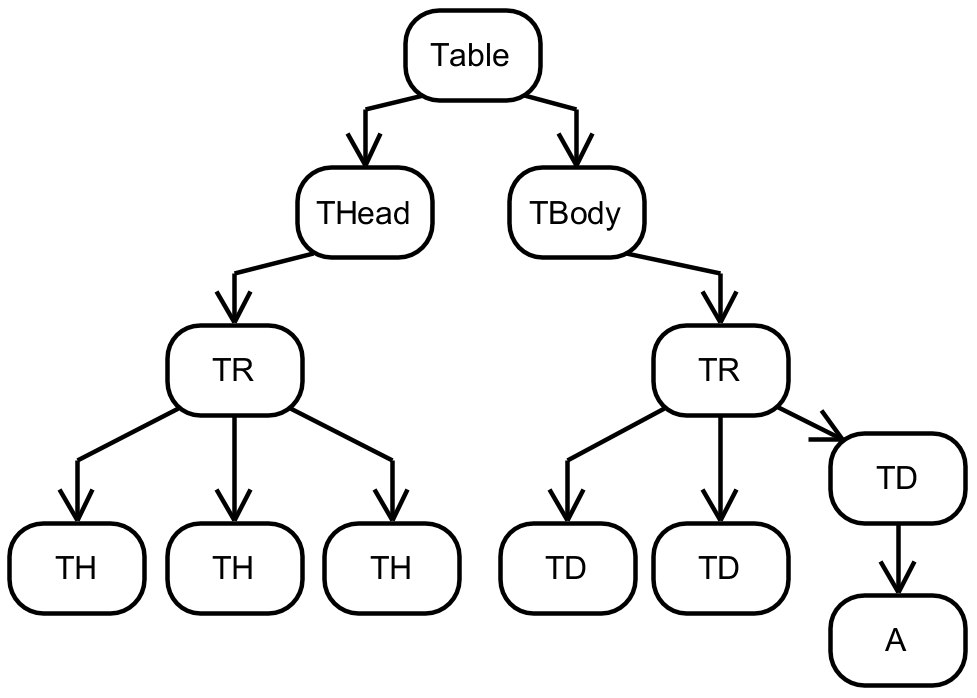
\includegraphics[width=\textwidth]{domTree.png}
			\end{column}
		\end{columns}
	\end{frame}

	\begin{frame}[fragile]
		\frametitle{HTML-формы}
		\begin{itemize}
			\item Способ получить ввод от пользователя
			\item Возможность организовать POST-запрос (GET по умолчанию)
		\end{itemize}
		\begin{minted}{html}
<form method="post">
  First name:<br>
  <input type="text" name="firstName"><br>
  Last name:<br>
  <input type="text" name="lastName"><br><br>
  <input type="radio" name="gender" value="male" checked>Male<br>
  <input type="radio" name="gender" value="female">Female<br>
  <input type="submit" value="Submit">
</form>
		\end{minted}
	\end{frame}

	\begin{frame}[fragile]
		\frametitle{CSS}
		\begin{itemize}
			\item Способ задать внешний вид элементов
		\end{itemize}
		\begin{minted}{html}
<!DOCTYPE html>
<html>
<head>
<style>
  body {background-color: powderblue;}
  h1   {color: blue;}
  p    {color: red;}
</style>
</head>
<body>
<h1>This is a heading</h1>
<p>This is a paragraph.</p>
</body>
</html>
		\end{minted}
		\attribution{https://www.w3schools.com}
	\end{frame}

	\begin{frame}[fragile]
		\frametitle{Или, что более типично}
		\begin{minted}{html}
<!DOCTYPE html>
<html>
<head>
  <link rel="stylesheet" href="styles.css">
</head>
<body>

<h1>This is a heading</h1>
<p>This is a paragraph.</p>

</body>
</html>
		\end{minted}
		\attribution{https://www.w3schools.com}
	\end{frame}

	\begin{frame}[fragile]
		\frametitle{Селекторы}
		\begin{minted}{html}
<p id="p01">I am different</p>
<p class="error">Error message</p>
		\end{minted}
		\vspace{5mm}
		\begin{minted}{css}
#p01 {
    color: blue;
}

p.error {
    color: red;
}
		\end{minted}
		\attribution{https://www.w3schools.com}
	\end{frame}

	\begin{frame}[fragile]
		\frametitle{Немного JavaScript-а}
		\begin{minted}{html}
<!DOCTYPE html>
<html>
<body>

<h1>My First JavaScript</h1>

<button type="button"
onclick="document.getElementById('demo').innerHTML = Date()">
Click me to display Date and Time.</button>

<p id="demo"></p>

</body>
</html> 
		\end{minted}
		\attribution{https://www.w3schools.com}
	\end{frame}

	\begin{frame}[fragile]
		\frametitle{Или так}
		\begin{small}
			\begin{minted}{html}
<!DOCTYPE html>
<html>
<head>
<script>
function doSomething() {
  document.getElementById("demo").style.fontSize = "25px";
  document.getElementById("demo").style.color = "red";
  document.getElementById("demo").style.backgroundColor = "yellow";
}
</script>
</head>
<body>

<button type="button" id="demo" onclick="doSomething()">Click me!</button>

</body>
</html>
			\end{minted}
		\end{small}
		\vspace{-3mm}
		\attribution{https://www.w3schools.com}
	\end{frame}

	\begin{frame}
		\frametitle{AJAX}
		\framesubtitle{Asynchronous JavaScript And XML}
		\begin{center}
			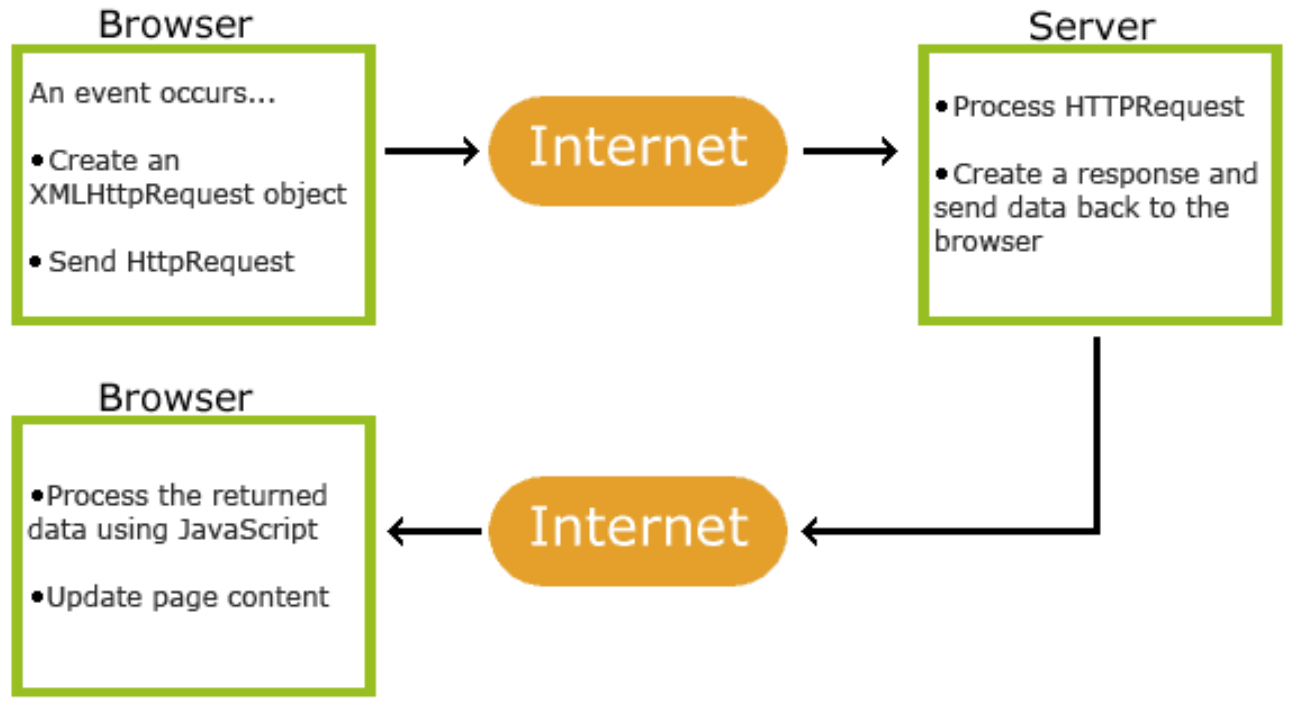
\includegraphics[width=0.7\textwidth]{ajax.png}
		\end{center}
	\end{frame}

	\begin{frame}[fragile]
		\frametitle{Пример}
		\begin{scriptsize}
			\begin{minted}{html}
<!DOCTYPE html>
<html>
<body>
<div id="demo">
  <h2>The XMLHttpRequest Object</h2>
  <button type="button" onclick="loadDoc()">Change Content</button>
</div>
<script>
function loadDoc() {
  var xhttp = new XMLHttpRequest();
  xhttp.onreadystatechange = function() {
    if (this.readyState == 4 && this.status == 200) {
      document.getElementById("demo").innerHTML =
      this.responseText;
    }
  };
  xhttp.open("GET", "ajax_info.txt", true);
  xhttp.send();
}
</script>
</body>
</html>
			\end{minted}
		\end{scriptsize}
		\vspace{-3mm}
		\attribution{https://www.w3schools.com}
	\end{frame}

	\section{Бэкенд}

	\begin{frame}
		\frametitle{Бэкенд}
		\framesubtitle{Обработка веб-запроса в Windows}
		\begin{center}
			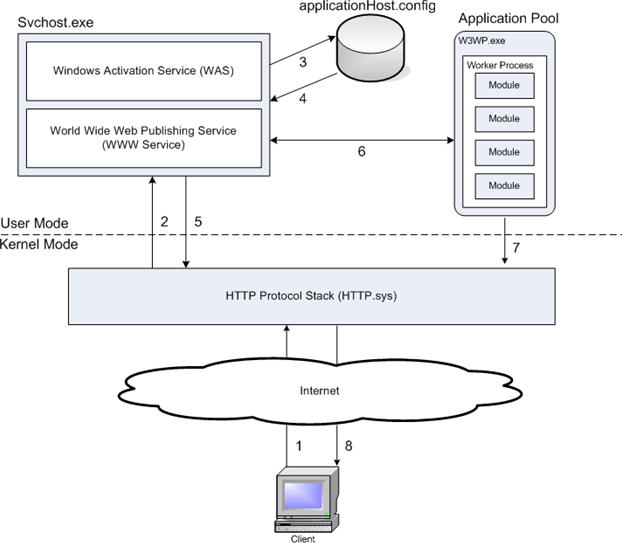
\includegraphics[width=0.65\textwidth]{requestProcessing.png}
			\vspace{-5mm}
			\attribution{MSDN}
		\end{center}
	\end{frame}

	\section{Архитектура ASP.NET MVC}

	\begin{frame}
		\frametitle{ASP.NET MVC, основные понятия}
		\begin{center}
			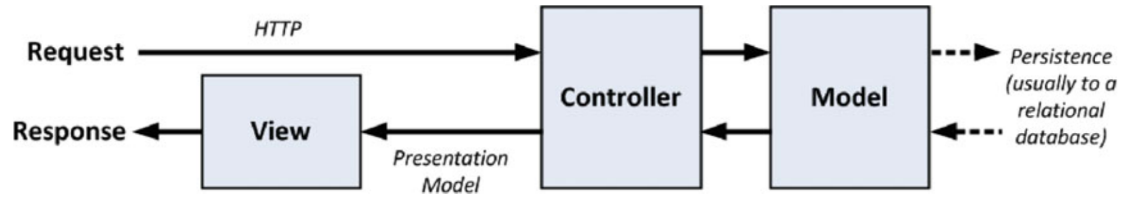
\includegraphics[width=0.7\textwidth]{mvc.png}
			\attribution{A. Freeman, Pro ASP.NET Core MVC}
		\end{center}

		\vspace{-5mm}

		\begin{itemize}
			\item \textbf{Модель} содержит или представляет данные, с которыми работает приложение
			\begin{itemize}
				\item \textbf{Domain model} содержит объекты предметной области вместе с бизнес-логикой, механизмами сериализации и т.д.
				\item \textbf{View Model} содержит классы, удобные для отображения во View, без бизнес-логики
			\end{itemize}
			\item \textbf{Представление} (View) отвечает за показ данных из модели пользователю
			\begin{itemize}
				\item Работает в браузере, но генерится на сервере
			\end{itemize}
			\item \textbf{Контроллер} отвечает за обработку входящих запросов, преобразование моделей и формирование данных для видов
		\end{itemize}
	\end{frame}

	\begin{frame}
		\frametitle{Обработка веб-запроса в ASP.NET}
		\begin{center}
			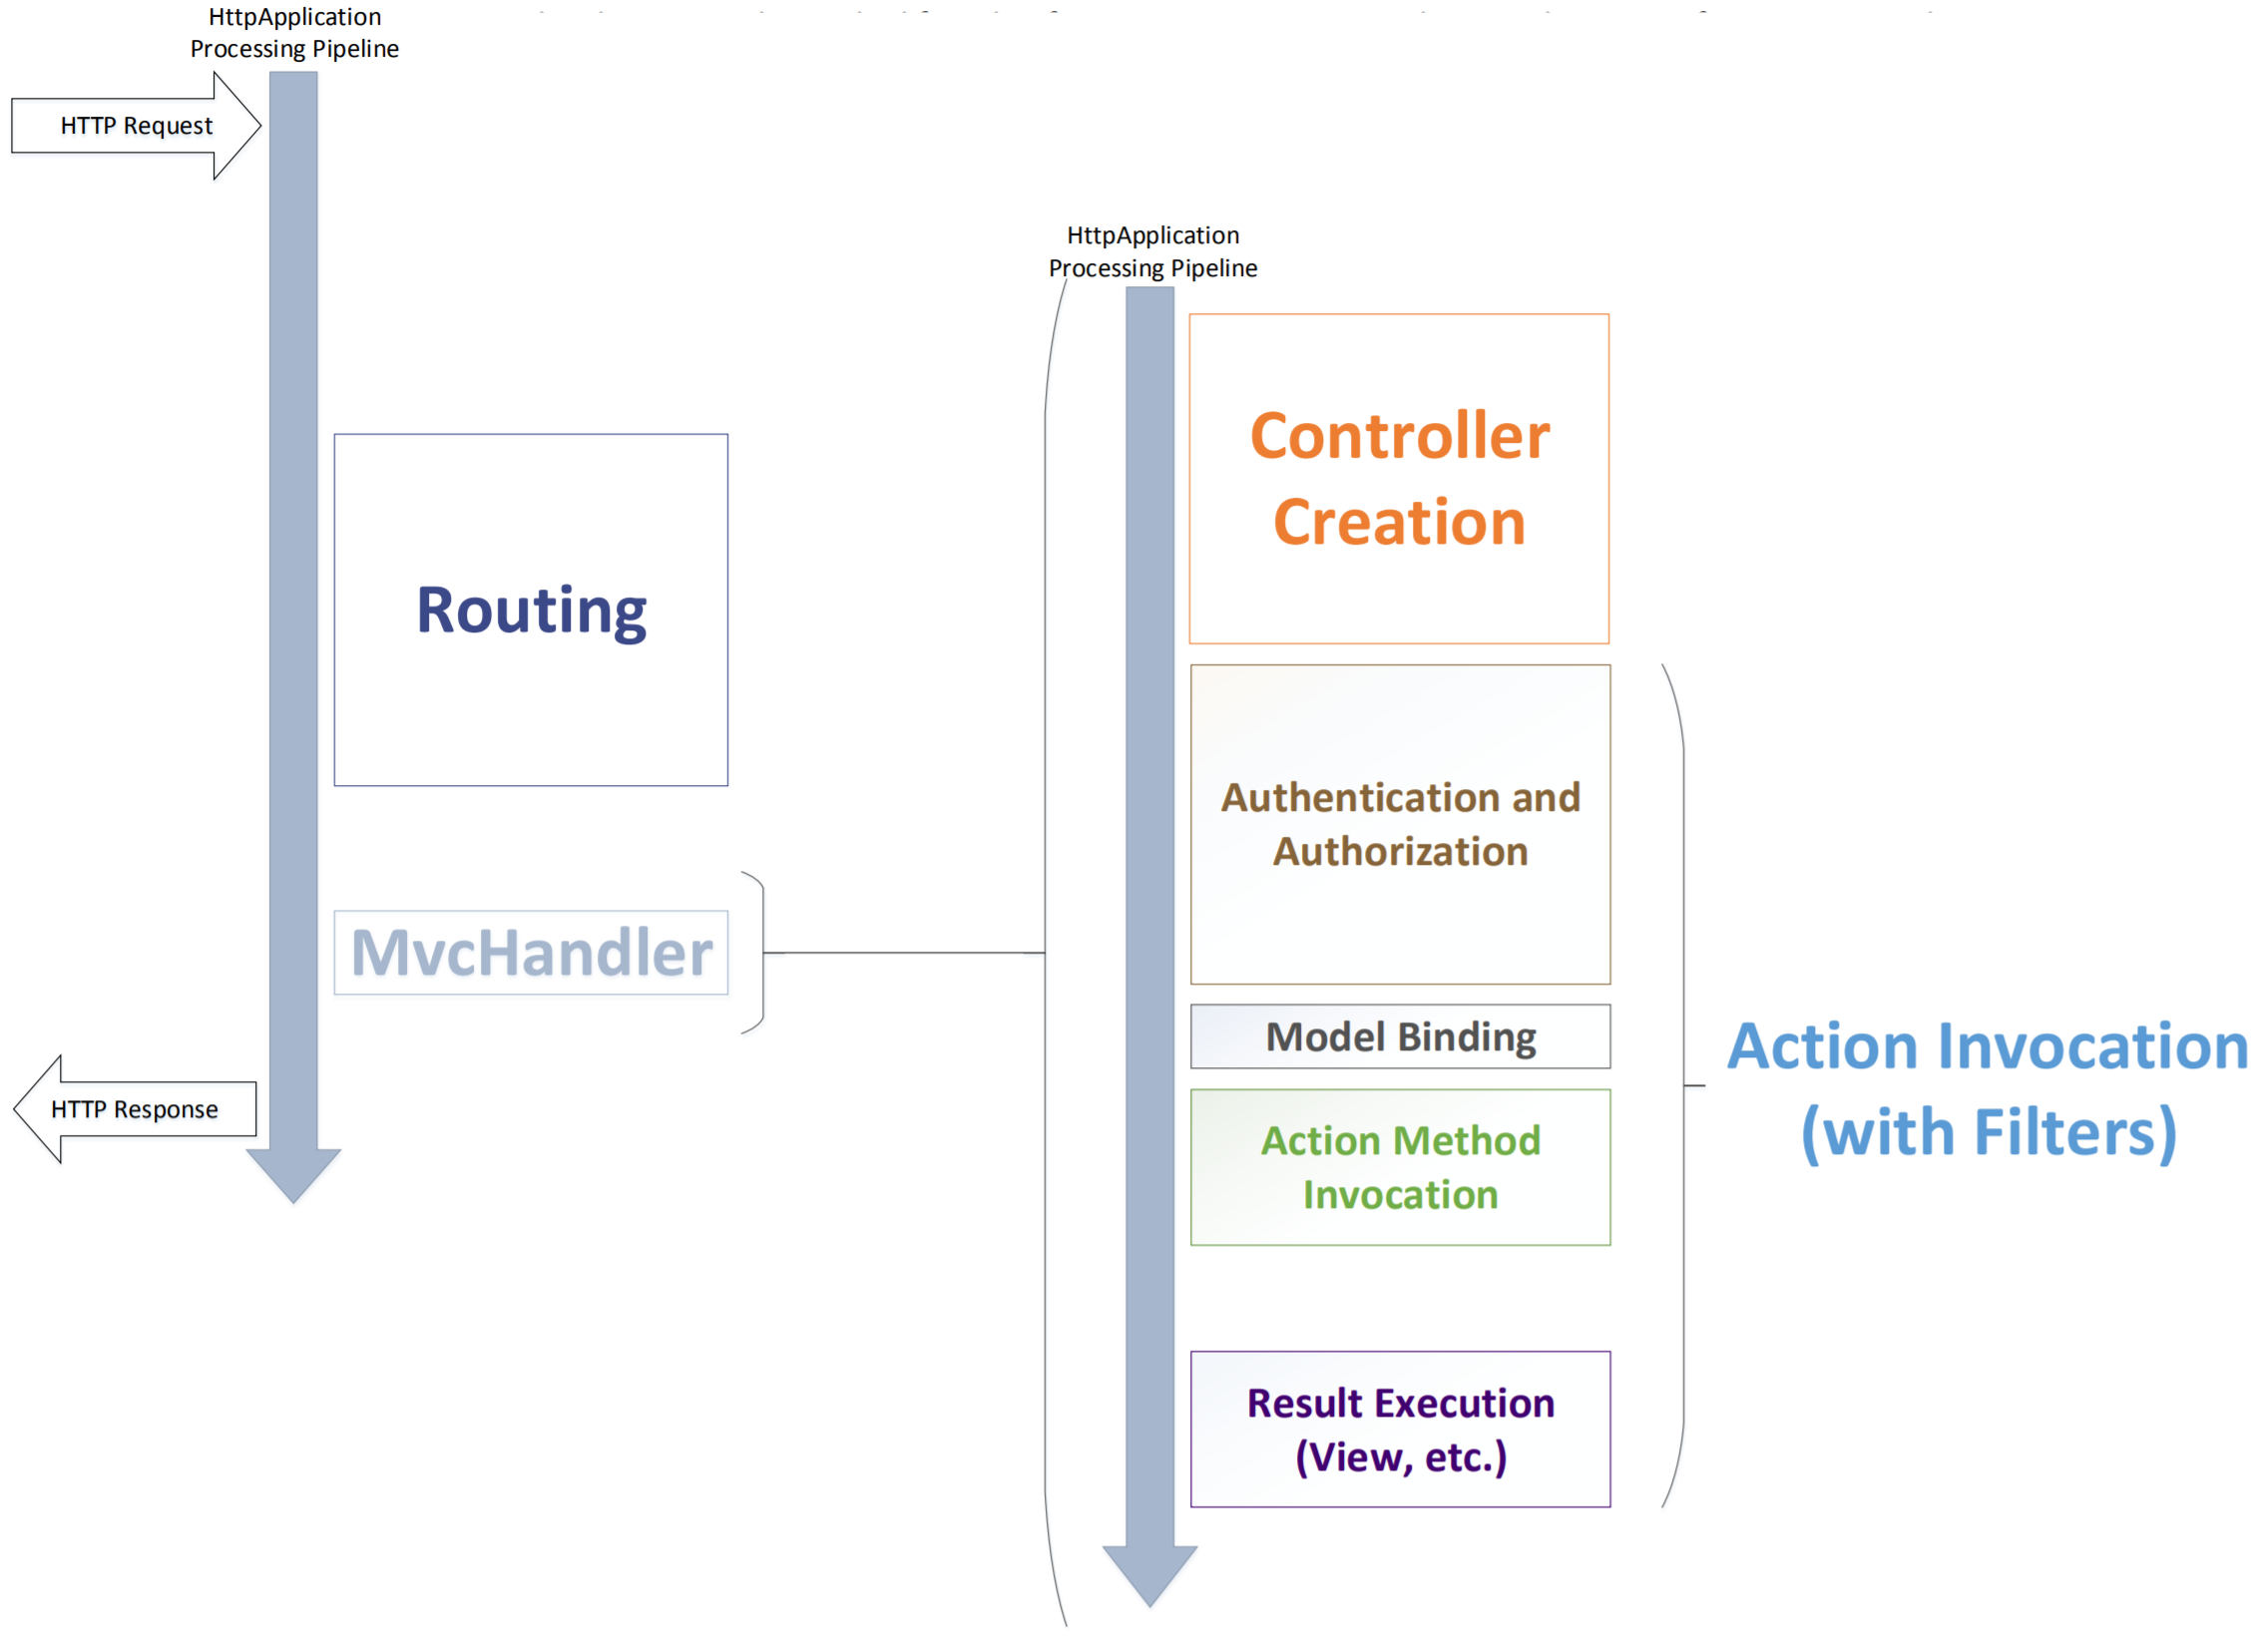
\includegraphics[width=0.85\textwidth]{requestLifecycle.png}
			\vspace{-5mm}
			\attribution{MSDN}
		\end{center}
	\end{frame}

\end{document}
